\section{Research Portfolio: 41 Papers Across Six Programs}
\label{sec:portfolio}

\begin{designbox}
Report the research output as a de-duplicated inventory, broken down by program
and by manuscript/draft status, compared only to human-authored literature and
baselines. Count what exists; claim no acceptances.
\end{designbox}

Beyond the benchmark arenas, Argus runs an optional idea-to-submission research
pipeline (the \code{research} vertical), which drives literature grounding,
experiment design, execution, results analysis, and manuscript writing through
per-stage checklists and a Reviewer peer-review gate. Its public output is a
collection of \textbf{41 papers}~\cite{argus_research}: 35 manuscripts and 6
drafts, with duplicate versions removed, across six research programs.
Figure~\ref{fig:portfolio} and Table~\ref{tab:portfolio} give the breakdown.

\begin{figure}[ht]
\centering
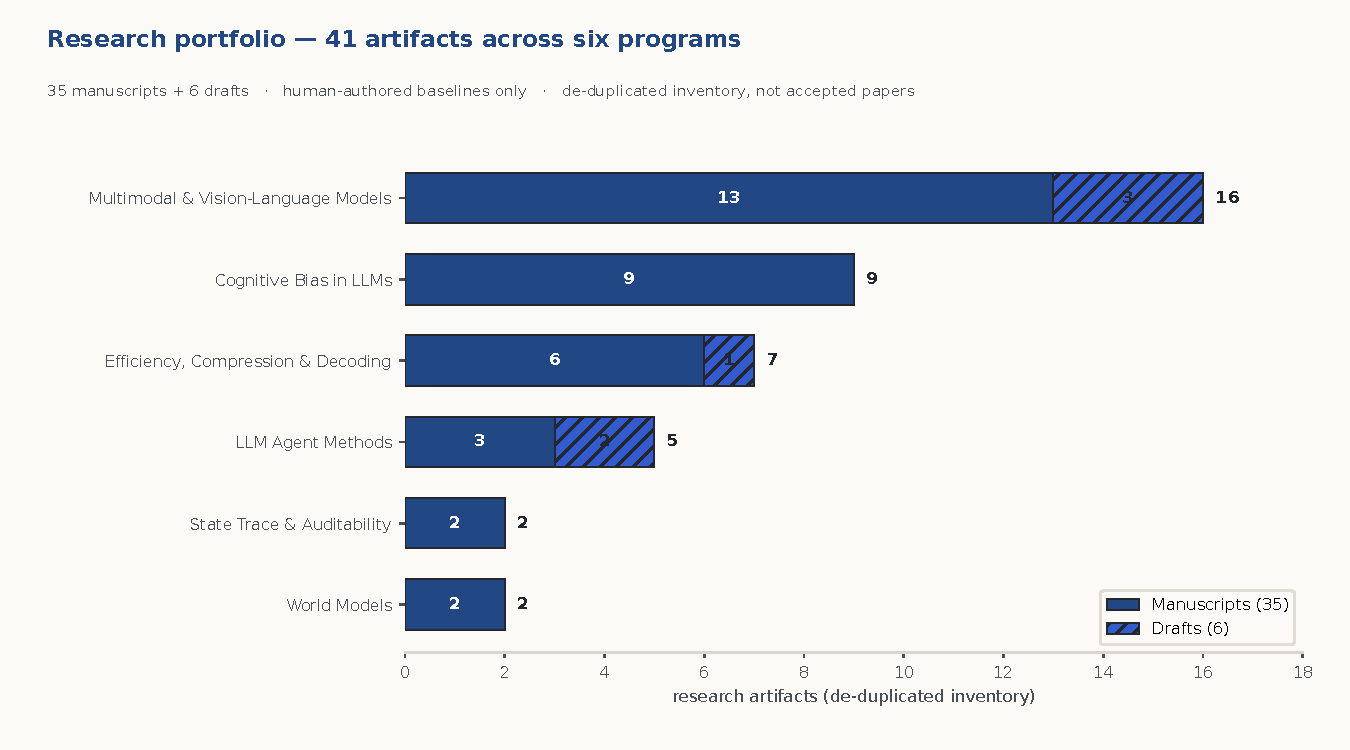
\includegraphics[width=\textwidth]{figures/paper_portfolio.pdf}
\caption{The 41-paper portfolio by program and status, drawn deterministically
from \code{technical\_report/evidence/paper\_inventory.json}. Manuscripts are
indigo, drafts lighter. The count is a de-duplicated inventory compared only to
human-authored literature/baselines --- not a count of accepted papers.}
\label{fig:portfolio}
\end{figure}

\begin{table}[h]
\centering
\small
\begin{tabularx}{\linewidth}{@{}X r r r@{}}
\toprule
\textbf{Program} & \textbf{Manuscripts} & \textbf{Drafts} & \textbf{Total} \\
\midrule
Multimodal \& Vision-Language Models & 13 & 3 & 16 \\
Cognitive Bias in LLMs               &  9 & 0 &  9 \\
Efficiency, Compression \& Decoding  &  6 & 1 &  7 \\
LLM Agent Methods                    &  3 & 2 &  5 \\
World Models                         &  2 & 0 &  2 \\
State Trace \& Auditability          &  2 & 0 &  2 \\
\midrule
\textbf{Total}                       & \textbf{35} & \textbf{6} & \textbf{41} \\
\bottomrule
\end{tabularx}
\caption{Research portfolio by program and status~\cite{argus_research}. The
machine-readable inventory is
\code{technical\_report/evidence/paper\_inventory.json}.}
\label{tab:portfolio}
\end{table}

\subsection{The six programs}

The portfolio concentrates in a few areas. \textbf{Multimodal \& Vision-Language
Models} is the largest program (16 papers), followed by \textbf{Cognitive Bias in
LLMs} (9), which studies train-free mitigation of biases such as anchoring,
base-rate neglect, and status-quo defaults. \textbf{Efficiency, Compression \&
Decoding} (7) covers inference-time methods; \textbf{LLM Agent Methods} (5) covers
agent techniques; and two smaller programs, \textbf{World Models} (2) and
\textbf{State Trace \& Auditability} (2), round out the set. Each paper is
positioned against human-authored literature and baselines; the human comparison,
where the site provides one, is preserved in the inventory.

\subsection{What the count means}

Three qualifications keep the number honest. First, 41 is a \emph{de-duplicated
inventory} of research runs that produced a manuscript or draft; it is not a count
of accepted papers, and this report makes no acceptance claim. Second, the
manuscript/draft split (35/6) is reported as-is: a draft is an in-progress
artifact, not a finished manuscript. Third, the collection is compared
\emph{only} to human-authored literature and baselines --- paper count and paper
quality are never compared to any other agent or model. The research pipeline is a
capability that produces auditable manuscripts under the same completion authority
as every other mission (Section~\ref{sec:roles}); it is not a claim that any of
those manuscripts has cleared external peer review.
